\documentclass[12pt, titlepage]{article}

\usepackage{amsmath, mathtools}

\usepackage[round]{natbib}
\usepackage{amsfonts}
\usepackage{amssymb}
\usepackage{graphicx}
\usepackage{colortbl}
\usepackage{xr}
\usepackage{hyperref}
\usepackage{longtable}
\usepackage{xfrac}
\usepackage{tabularx}
\usepackage{float}
\usepackage{siunitx}
\usepackage{booktabs}
\usepackage{multirow}
\usepackage[section]{placeins}
\usepackage{caption}
\usepackage{fullpage}
\usepackage{makecell}

\hypersetup{
bookmarks=true,     % show bookmarks bar?
colorlinks=true,       % false: boxed links; true: colored links
linkcolor=red,          % color of internal links (change box color with linkbordercolor)
citecolor=blue,      % color of links to bibliography
filecolor=magenta,  % color of file links
urlcolor=cyan          % color of external links
}

\usepackage{array}

\externaldocument{../../SRS/SRS}


\begin{document}

\title{Module Interface Specification for Retinal Vessel Segmentation System (RVSS)}

\author{Xinyu Ma}

\date{March 18, 2024}

\maketitle

\pagenumbering{roman}

\section{Revision History}

\begin{tabularx}{\textwidth}{p{3cm}p{2cm}X}
\toprule {\bf Date} & {\bf Version} & {\bf Notes}\\
\midrule
03/14/2024 & 1.0 & Initial Release  \\
03/18/2024 & 2.0 & Add some flow charts  \\
\bottomrule
\end{tabularx}

~\newpage

\section{Symbols, Abbreviations and Acronyms}

See \href{https://github.com/lele0007/Blood-vessel-segmentation/blob/main/docs/SRS/SRS.pdf}{SRS} Documentation for symbols, abbreviations and acronyms. \\ 

\renewcommand{\arraystretch}{1.2}
\begin{tabular}{l l} 
  \toprule		
  \textbf{symbol} & \textbf{description}\\
  \midrule 
  CNN & Convolution Neural Network\\
  DAG & Directed Acyclic Graph \\
  M & Module \\
  MG & Module Guide \\
  OS & Operating System \\
  R & Requirement\\
  RVSS & Retinal Vessel Segmentation System \\ 
  SRS & Software Requirements Specification\\
  \bottomrule
\end{tabular}\\

\newpage

\tableofcontents

\listoftables

\newpage

\pagenumbering{arabic}

\section{Introduction}

The following document details the Module Interface Specifications for
Retinal Vessel Segmentation System (RVSS). This document specifies how every module is interfacing with every other parts. 

Complementary documents include the \href{https://github.com/lele0007/Blood-vessel-segmentation/blob/main/docs/SRS/SRS.pdf}{System Requirement Specifications}
and \href{https://github.com/lele0007/Blood-vessel-segmentation/blob/main/docs/Design/SoftArchitecture/MG.pdf}{Module Guide}.  The full documentation and implementation can be
found at \href{https://github.com/lele0007/Blood-vessel-segmentation.git}{Github repository for RVSS}.

\section{Notation}


The structure of the MIS for modules comes from \citet{HoffmanAndStrooper1995},
with the addition that template modules have been adapted from
\citet{ghezzi1991fundamentals}.  The mathematical notation comes from Chapter 3 of
\citet{HoffmanAndStrooper1995}.  For instance, the symbol := is used for a
multiple assignment statement and conditional rules follow the form $(c_1
\Rightarrow r_1 | c_2 \Rightarrow r_2 | ... | c_n \Rightarrow r_n )$.

The following table summarizes the primitive data types used by SCEC. 

\begin{center}
\renewcommand{\arraystretch}{1.2}
\noindent 
\begin{tabular}{l l p{7.5cm}} 
\toprule 
\textbf{Data Type} & \textbf{Notation} & \textbf{Description}\\ 
\midrule
character & char & a single symbol or digit\\
integer & $\mathbb{Z}$ & a number without a fractional component in (-$\infty$, $\infty$) \\
natural number & $\mathbb{N}$ & a number without a fractional component in [1, $\infty$) \\
real & $\mathbb{R}$ & any number in (-$\infty$, $\infty$)\\
Boolean & $\mathbb{B}$ & a value of either True or False\\
\bottomrule
\end{tabular} 
\end{center}

\noindent
The specification of RVSS uses some derived data types: sequences, strings, and
tuples. Sequences are lists filled with elements of the same data type. Strings
are sequences of characters. Tuples contain a list of values, potentially of
different types. In addition, RVSS uses functions, which
are defined by the data types of their inputs and outputs. Local functions are
described by giving their type signature followed by their specification.

\section{Module Decomposition}

The following table is taken directly from the Module Guide document for this project.

\begin{table}[h!]
\centering
\begin{tabular}{p{0.3\textwidth} p{0.6\textwidth}}
\toprule
\textbf{Level 1} & \textbf{Level 2}\\
\midrule
{Hardware-Hiding Module} & ~ \\
\midrule

\multirow{7}{0.3\textwidth}{Behaviour-Hiding Module} 
& Input Upload and Validate Module\\ 
& Image Management Module\\
& Image Preprocessing Module\\
& Image Segmentation Module\\
& Output Format Module\\
& Report Generation Module\\
& User Interface Module\\
& Main Function Module\\
\midrule

\multirow{3}{0.3\textwidth}{Software Decision Module} 
& Algorithm Optimization Module\\
& Plotting Result Module\\
& Logging Module\\
& Image patching Module\\
& Image Dataset Reader Module\\
& Network Model Reader Module\\
\bottomrule

\end{tabular}
\caption{Module Hierarchy}
\label{TblMH}
\end{table}


\newpage
~\newpage

\section{MIS of Input Upload and Validate Module} \label{m1} 

\subsection{Module}

UploadValidate

\subsection{Uses}
\begin{itemize}
    \item Image Management Module
\end{itemize}
\subsection{Syntax}

\subsubsection{Exported Constants}
\begin{itemize}
    \item Accpted$\_$Image$\_$Formats: list of image file formats that the system can process (e.g., [".jpg", ".jpeg", ".png"]).
    \item Max\_Image\_Size: maximum file size for uploaded images, specified in megabytes.
    \item Min\_Image\_Resolution: minimum image resolution required for processing, specified as (width, height) in pixels.
\end{itemize}
\subsubsection{Exported Access Programs}
1. UploadImage
\begin{itemize}
    \item Description: receives and stores an image file uploaded by the user.
    \item Input: an image file representing the retinal image.
    \item Output: upload success or fail (data type: boolean); ImageID (string if uploading successfully).
    \item Exceptions: ``UploadFailureException" if the upload process fails due to system issues.
\end{itemize}
2. ValidateImage
\begin{itemize}
    \item Description: validates the uploaded image to ensure it meets the system's criteria for format, size, and quality.
    \item Input: ImageID (unique identifier for the uploaded image).
    \item Output: Validation Result (object containing validation status and any issues found).
    \item Exceptions: ``ImageNotFoundException" if the image corresponding to the ImageID cannot be found, and ``ValidationException" if the image does not match the predefined criteria.
\end{itemize}

\subsection{Semantics}

\subsubsection{State Variables}
Uploaded\_Images\_Data: a collection or database table reference storing information about uploaded images, including their temporary IDs, upload status, and validation status.


\subsubsection{Environment Variables}
Upload\_Path: the file system path to the directory where uploaded images are temporarily stored.

\subsubsection{Assumptions}

None

\subsubsection{Access Routine Semantics}
1. UploadImage
\begin{itemize}
    \item Transition: accepts an image file (``imageFile") uploaded by the user. The routine stores the image temporarily in the system and assigns it a unique ``ImageID", then updates the ``UploadedImagesData" state variable to include the new image and its upload status. The image is saved to the temporary storage area specified by the ``Upload\_Path" environment variable.
    \item Exceptions: ``UploadFailureException" raised if the upload process fails due to system issues.
\end{itemize}
2. ValidateImage
\begin{itemize}
    \item Transition: takes a ``ImageID" as input and retrieves the corresponding image from ``Uploaded\_Images\_Data". Then validates the image against predefined criteria such as format, size, and resolution. The ``UploadedImagesData" state variable is updated to reflect the validation status of the image.
    \item Exceptions: ``ImageNotFoundException" raised if no image matches the provided ``ImageID". ``ValidationException" raised if an error occurs during the validation process.
\end{itemize}

\subsubsection{Local Functions}

None



\newpage

\section{MIS of Image Management Module} \label{m2} 
For each retina image uploaded by users, a unique ImageID will be assigned. The ImageID, original image, image upload verification status, image preprocessing status, image segmentation status, and image segmentation result are stored as one item, and all image status can be accessed using only the ImageID.
\subsection{Module}

ImageManagement

\subsection{Uses}
None

\subsection{Syntax}

\subsubsection{Exported Constants}
None

\subsubsection{Exported Access Programs}
1. StoreImage
\begin{itemize}
    \item Input: image data (type: Tensor)
    \item Output: ImageID which is a unique identifier for the stored image.
    \item Exceptions: ``StorageException" raised if failure occurs during the image storage process.
\end{itemize}

2. RetrieveImage
\begin{itemize}
    \item Input: ImageID
    \item Output: data of the retrieved image.
    \item Exceptions: ``ImageNotFoundException" raised if no image matches the ImageID, and ``RetrievalException" raised if failure happens during the image retrieval process.
\end{itemize}



\subsection{Semantics}

\subsubsection{State Variables}
ImageDatabase: A data structure that keeps track of all stored images, their state, and ImageID. This could be an in-memory structure or a connection to an external database system.

\subsubsection{Environment Variables}

Storage\_Path: specifies the filesystem path to the directory where images are stored.

\subsubsection{Assumptions}

None 

\subsubsection{Access Routine Semantics}
1. StoreImage
\begin{itemize}
    \item Transition:Saves the provided image to the storage system, then generates a unique ImageID for the image, which is used for future retrieval or reference. Updates ImageDatabase by adding a new entry for the stored image, including its storageID and associated state.
    \item Exceptions: ``StorageException" raised if failure occurs during the image storage process.
\end{itemize}
\begin{figure}[H]
\centering
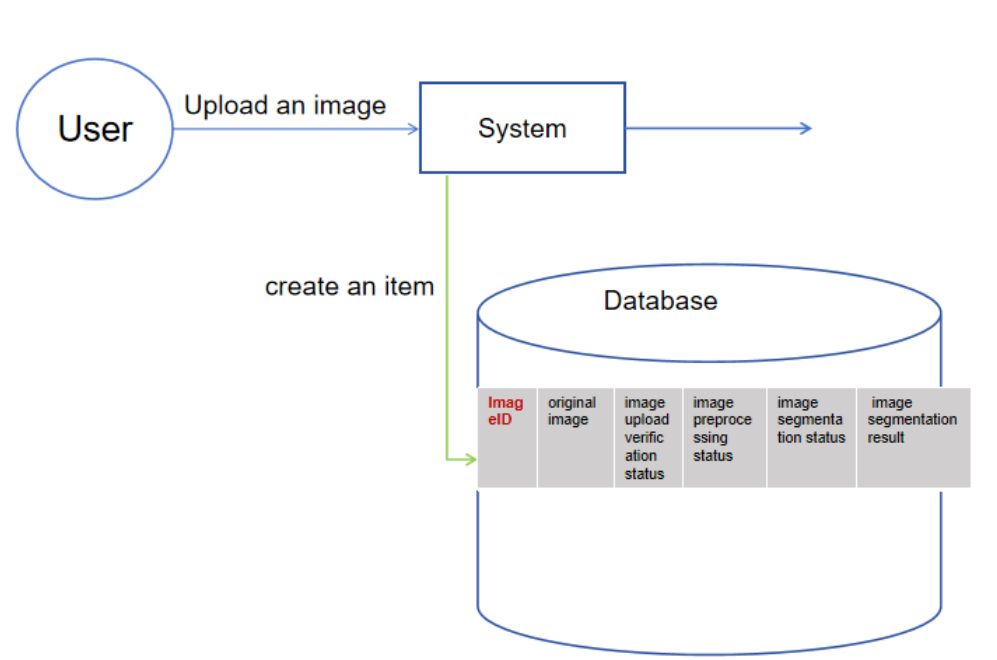
\includegraphics[width=0.5\textwidth]{2.png}
\caption{Store Image}
\label{Fig1}
\end{figure}

2. RetrieveImage
\begin{itemize}
    \item Transition: ImageID is provided, then retrieves the specific image and its state associated with the ImageID.

    \item Exceptions: ``ImageNotFoundException" raised if no image matches the ImageID, and ``RetrievalException" raised in case of failures during the retrieval process.

\begin{figure}[H]
\centering
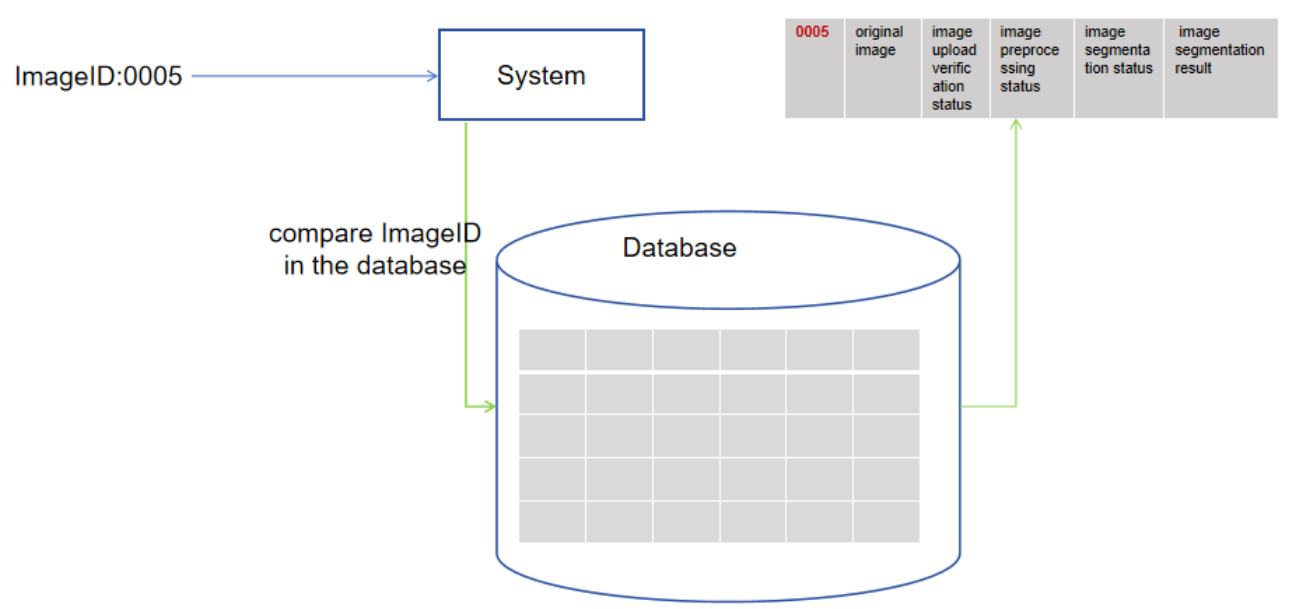
\includegraphics[width=0.5\textwidth]{3.png}
\caption{Retrieve an image}
\label{Fig2}
\end{figure}


\subsubsection{Local Functions}
None

\newpage

\section{MIS of Image Preprocessing Module} \label{m3} 

\subsection{Module}

ImagePreprocessing

\subsection{Uses}

\begin{itemize}
    \item Image Management Module
\end{itemize}

\subsection{Syntax}

\subsubsection{Exported Constants}
\begin{itemize}
    \item Normalization\_Range: defines the target range for image intensity normalization, e.g., [0, 1] or [0, 255].
    \item Denoising\_Strength: a predefined level or parameter settings for the denoising algorithm.
    \item Contrast \_Enhancement \_Parameters: a parameter that controls the degree of contrast enhancement applied to images.
\end{itemize}

\subsubsection{Exported Access Programs}
1. NormalizeImage
\begin{itemize}
    \item Inputs: ImageID
    \item Outputs: the image with intensity values normalized.
    \item Exceptions:``NormalizationException" raised if normalization fails, and ``ImageNotFoundException” raised if no image matches the ImageID.
\end{itemize}

2. DenoiseImage
\begin{itemize}
    \item Inputs: ImageID
    \item Outputs: the image with reduced noise.
    \item Exceptions: ``DenoisingException" raised if denoising fails.
\end{itemize}

3. EnhanceImageContrast
\begin{itemize}
    \item Inputs: ImageID
    \item Outputs: the image with with enhanced contrast.
    \item Exceptions:``ContrastEnhancementException" raised if enhancement fails.
\end{itemize}


\subsection{Semantics}

\subsubsection{State Variables}

None

\subsubsection{Environment Variables}

None


\subsubsection{Assumptions}

\begin{itemize}
    \item Consistent preprocessing parameters: there's an assumption that preprocessing parameters (e.g., normalization range, denoising strength) are chosen to be effective across the spectrum of images processed by the system. While parameters might be adjustable, the defaults are assumed to be generally applicable.

    \item Image preprocessing steps: For an image, first normalize the image, then denoise, and finally enhance the contrast.
\end{itemize}

\subsubsection{Access Routine Semantics}
1. NormalizeImage
\begin{itemize}
    \item Transition: use the ``ImageID" to retrieve images in the Image Database, then adjusts the intensity values of the raw image to fall within a specified range, enhancing uniformity across images for improved segmentation performance. Store the normalized image in the Image Database.
    \item Exceptions:``NormalizationException" if normalization fails due to unexpected image properties, and ``ImageNotFoundException” raised if no image matches the ImageID.
\end{itemize}

2. DenoiseImage
\begin{itemize}
    \item Transition: use the ``ImageID" to retrieve images in the Image Database, then check whether the image has been normalized. If the image has a normalized version, then applies a denoising algorithm to it to reduce noise while preserving essential details, crucial for accurate segmentation. Store the normalized image in the Image Database.
    \item Exceptions:``DenoisingException" raised if denoising is unsuccessful or leads to significant loss of image detail.
\end{itemize}

3. EnhanceImageContrast
\begin{itemize}
    \item Transition: use the ``ImageID" to retrieve images in the Image Database, then check whether the image has been denoised. If the image has a denoised version, then using methods suited to highlight features relevant to vessel segmentation, potentially making vessels more distinct. Store the contrast enhanced image in the Image Database.
    \item Outputs: The image with with enhanced contrast.
    \item Exceptions:``ContrastEnhancementException" raised if the process fails or results in an unusable image.
\end{itemize}

\begin{figure}[H]
\centering
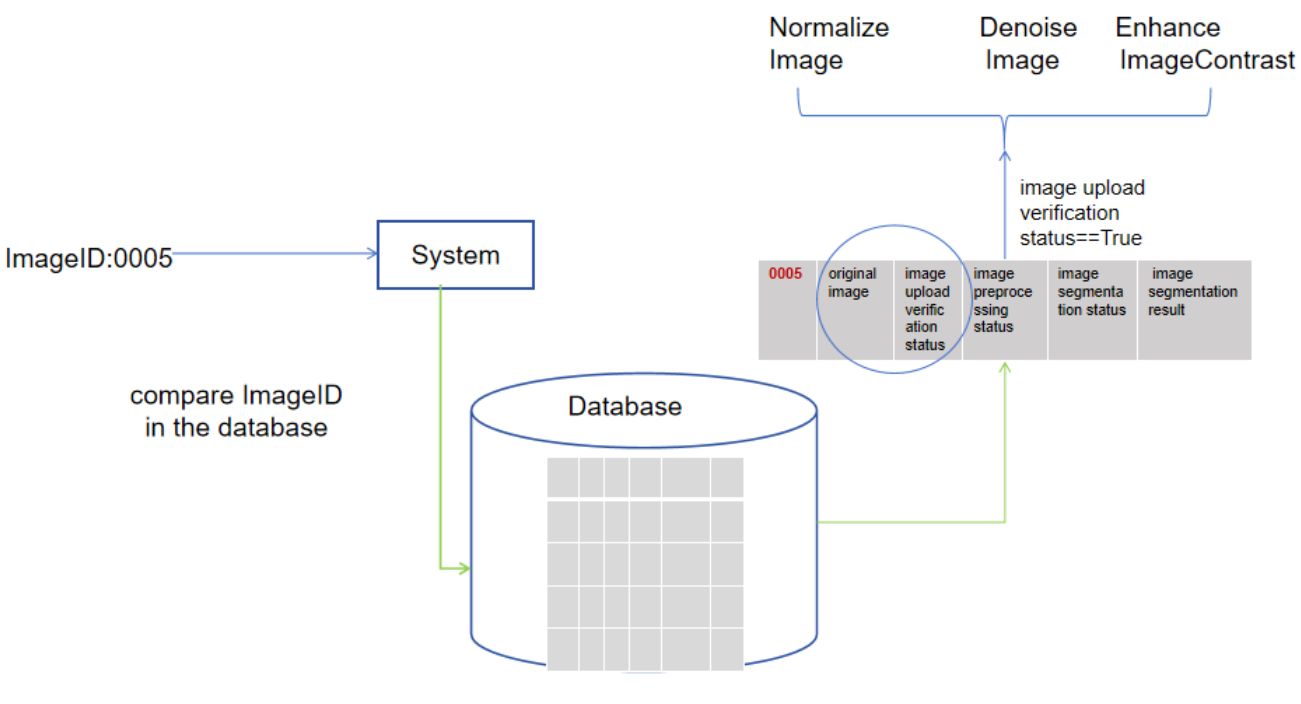
\includegraphics[width=0.5\textwidth]{4.png}
\caption{Image Preprocessing Module}
\label{Fig3}
\end{figure}
\subsubsection{Local Functions}
None


\newpage
\section{MIS of Image Segmentation Module} \label{m4} 

\subsection{Module}
ImageSegmentation

\subsection{Uses}

\begin{itemize}
    \item Image Management Module
    \item Image Preprocessing Module
\end{itemize}

\subsection{Syntax}

\subsubsection{Exported Constants}
Segmentation\_Algorithm: Specifies the default algorithm or model used for image segmentation. It could be a string identifier or algorithm-specific parameters.

\subsubsection{Exported Access Programs}
1. SegmentImage
\begin{itemize}
    \item Description: performs segmentation on a preprocessed image to identify and delineate retinal vessels.
    \item Input: ImageID
    \item Output: prompt message that image segmentation is completed 
    \item Exceptions: ``PreprocessedImageNotFoundException" raised if the preprocessed image corresponding to the ImageID cannot be found, and ``SegmentationException raised if the segmentation process encounters errors.
\end{itemize}


\subsection{Semantics}
\subsubsection{State Variables}
Current\_Algorithm\_Settings: Stores the current settings or parameters used by the segmentation algorithm, allowing for adjustments if needed.

\subsubsection{Environment Variables}

Model\_Storage\_Path: The filesystem path pointing to the location where segmentation models or algorithm parameters are stored, enabling the module to dynamically load different models based on system configuration or needs.

\subsubsection{Assumptions}
\begin{itemize}
    \item The input images are preprocessed and normalized, ensuring consistency in image quality and format that is conducive to effective segmentation.
    \item The segmentation algorithms or models are pre-trained, capable of delivering high accuracy in vessel delineation across diverse image datasets.
\end{itemize}

\subsubsection{Access Routine Semantics}

1. SegmentImage
\begin{itemize}
\item Transition: use the``ImageID” to retrieve images in the Image Database, then check
whether the image has been preprocessed. Takes the preprocessed image and applies the segmentation algorithm defined by Segmentation\_Algorithm and Current\_Algorithm\\\_Settings, producing a prompt message when the image segmentation is completed. Stores the segmented image in the Image Database and logs related to segmentation performance.

\item Exception:  ``PreprocessedImageNotFoundException" raised if the preprocessed image corresponding to the ImageID cannot be found, and ``SegmentationException raised if the segmentation process encounters errors.
\end{itemize}

\end{itemize}

\subsubsection{Local Functions}
1. LoadSegmentationModel
\begin{itemize}
    \item Description: loads the segmentation model or algorithm parameters from storage and it is primarily called within SegmentImage before applying the segmentation algorithm.
    \item Input: None 
    \item Output: Model or algorithm parameters ready for use in segmentation.
\end{itemize}





\newpage
\section{MIS of Output Format Module} \label{m5}

\subsection{Module}
OutputFormat

\subsection{Uses}
\begin{itemize}
    \item Image Management Module

\end{itemize}

\subsection{Syntax}

\subsubsection{Exported Constants}
None 
\subsubsection{Exported Access Programs}
1.OutputSegmentationImage
\begin{itemize}
    \item Description: Output retinal image segmentation results.
    \item Input: ImageID
    \item Output: the corresponding segmented image
    \item Exceptions: “SegmentationImageNotFoundException” raised if the segmentation result corresponding to the ImageID cannot be found.
\end{itemize}

\subsection{Semantics}

\subsubsection{State Variables}
None

\subsubsection{Environment Variables}
Default\_Output\_Path: Specifies the default filesystem path where output images are saved if no specific path is provided in the request. This ensures that generated images are stored in a consistent location.

\subsubsection{Assumptions}
None
   
\subsubsection{Access Routine Semantics}
1. output
\begin{itemize}
\item Transition: This module is able to output the segmentation result. Use the``ImageID” to retrieve images in the Image Database, then check whether the image has been segmented. Then shows the segmentation image on the screen and store the image in Default\_Output\_Path.

\item Exception:  ``SegmentationImageNotFoundException" raised if the segmented image corresponding to the ImageID cannot be found.
\end{itemize}

\subsubsection{Local Functions}

None


\newpage
\section{MIS of Report Generation Module} \label{m6} 

\subsection{Module}

ReportGeneration

\subsection{Uses}

\begin{itemize}
    \item Image Management Module
    \item Output Format Module
\end{itemize}

\subsection{Syntax}

\subsubsection{Exported Constants}
None
\subsubsection{Exported Access Programs}

1. ReportGeneration
\begin{itemize}
    \item Description: Creates a comprehensive report that includes the segmentation results along with metrics relevant to the segmentation process.
    \item Input: ImageID
    \item Output: a document file that contains the generated report,
    \item Exceptions: “ImageNotFoundException” raised if the image corresponding to the ImageID cannot be found. ``ReportGenerationException": raised if there is an error during the report generation process, including issues with input data integrity or problems creating the document file.
\end{itemize}

\subsection{Semantics}

\subsubsection{State Variables}
\begin{itemize}
    \item Current\_Report\_Data: This variable holds the data currently being processed for report generation. It could be structured to include segmentation results, and any additional information that will be included in the final report
    \item Generated\_Reports: A collection or history of reports that have been generated during a session or over a specified period. This could be used for tracking, auditing, or re-generation purposes.
\end{itemize}

\subsubsection{Environment Variables}

\begin{itemize}
    \item Report\_Output\_Path: specifies the default filesystem path where generated report files are saved. This ensures that reports are stored in a consistent and retrievable location.
    \item Default\_Report\_Format: indicates the default format for reports generated by the module, used if no specific format is requested. This variable ensures consistency in report presentation and can be set based on user or system preferences.

\end{itemize}

\subsubsection{Assumptions}
\begin{itemize}
    \item The input segmentation result is complete and correctly formatted, ensuring that all necessary data for report generation is available and accurate.
    \item A suitable report template is available and correctly formatted, allowing for the dynamic insertion of analysis results.
    \item The system has access to the necessary resources and permissions to create and save the report document in the specified format.
\end{itemize}

\subsubsection{Access Routine Semantics}
1. ReportGeneration
\begin{itemize}
\item Transition: Utilizing the ``ImageID" to retrieve images in the Image Database. It should include the original image, and the segmentation results along with metrics relevant to the segmentation process. Then use the Default\_Report\_Format to generate the report and save it according to the Report\_Output\_Path. 

\item ``UnsupportedFormatException": triggered if the requested report format is not among those supported by the system. “ImageNotFoundException” raised if the image corresponding to the ImageID cannot be found. ``ReportGenerationException": raised in cases where the report generation process encounters errors, such as template processing issues, data format problems, or file saving errors.
\end{itemize}


\subsubsection{Local Functions}
None









\newpage


\section{MIS of User Interface Module} \label{m7} 

\subsection{Module}

UI

\subsection{Uses}

\begin{itemize}
    \item Input Upload and Validate Module
    \item Image Management Module
    \item Image Preprocessing Module
    \item Image Segmentation Module
    \item Output Format Module
    \item Report Generation Module
\end{itemize}

\subsection{Syntax}

\subsubsection{Exported Constants}
\begin{itemize}
    \item Supported\_Image\_Formats: a list of image file formats that can be uploaded.
    \item Default\_Report\_Format:the default format for generated reports.
\end{itemize}
\subsubsection{Exported Access Programs}

1. Display Main Interface
\begin{itemize}
    \item Description: Presents the main interface screen to the user, offering access to various functionalities like image upload, segmentation, and report generation.
    \item Input: None
    \item Output: displays the main interface to the user.
    \item Exceptions: None
\end{itemize}
2. Upload Image Interface
\begin{itemize}
    \item Description: provides an interface for users to upload images for segmentation. 
    \item Input: user-selected image files.
    \item Output: confirmation of successful upload or feedback on any issues encountered, and a unique ImageID if uploading successfully.
    \item Exceptions: ``UploadFailureException” raised if there's an issue with uploading the image.
\end{itemize}

3. Segmentation Initiation
\begin{itemize}
    \item Description: triggers the segmentation process for uploaded images and displaying progress.
    \item Input: identifiers for images uploaded (``ImageID") and ready for segmentation.
    \item Output: status feedback during segmentation.
Notification upon completion or if issues arise.
    \item Exceptions: ``SegmentationInitiationException": raised if the segmentation process cannot be initiated .
\end{itemize}

4. View Segmentation Results
\begin{itemize}
    \item Description: displays segmentation results for selected images.
    \item Input: identifiers for images (``ImageID") whose segmentation results are to be viewed.
    \item Output: a display of segmentation results.
    \item Exceptions: ``ResultsDisplayException": raised if there's an issue retrieving or displaying results.
\end{itemize}

5. Generate Report
\begin{itemize}
    \item Description: facilitates the generation of reports based on segmentation results.
    \item Input: identifiers for images (``ImageID") and segmentation results to be included in the report.
    \item Output: a report file.
    \item Exceptions: ``ReportGenerationException": raised if report generation fails.
\end{itemize}

\subsection{Semantics}

\subsubsection{State Variables}
\begin{itemize}
    \item Current\_Screen: Tracks which interface screen is currently being displayed.
    \item Uploaded\_Images: A list of images that have been uploaded and are available for processing.
\end{itemize}

\subsubsection{Environment Variables}

\begin{itemize}
    \item Max\_Upload\_Size: defines the maximum size allowed for image uploads.
\end{itemize}

\subsubsection{Assumptions}
\begin{itemize}
    \item Users have a basic understanding of how to interact with web or desktop applications.
    \item The system is running on a platform capable of supporting graphical user interfaces (GUIs).
\end{itemize}

\subsubsection{Access Routine Semantics}
1. Display Main Screen
\begin{itemize}
    \item Purpose: To present the primary interface through which users interact with the system, offering navigation to various functionalities.
    \item Output: The main UI screen is displayed to the user and ensures that all primary functionalities (e.g., image upload, segmentation, report generation) are accessible.
    \item Exceptions: None
\end{itemize} 

2. Upload Image Interface
\begin{itemize}
    \item Purpose: provides a  mechanism for uploading images to be processed, including file selection dialogs.
    \item Transitions: validates the uploaded files and give a unique ImageID if uploading successfully. Displays progress and confirms once uploads are complete or provides error feedback. 
    \item Exceptions: ``UploadFailureException" which is triggered by issues like file size exceeding limits or unsupported formats.
\end{itemize} 

3. Segmentation  Initiation
\begin{itemize}
    \item Purpose: allows users to start the segmentation process for uploaded images.
    \item Transitions: initiates the process, and provides feedback on progress. Notifies the user upon completion or in case of errors.
    \item Exceptions: ``SegmentationInitiationException": raised if segmentation cannot be initiated.
\end{itemize} 


4. View Segmentation Results
\begin{itemize}
    \item Purpose: displays the results of image segmentation.
    \item Transitions: retrieves segmentation results according to the ``ImageID" and provide a display interface showing segmentation results..
    \item Exceptions: ``ResultsDisplayException": raised if there's a failure in retrieving or displaying the segmentation results, such as missing data or rendering issues
\end{itemize}

5. Generate Report
\begin{itemize}
    \item Purpose: enables users to generate comprehensive reports based on segmentation results.
    \item Transitions: retrieves original image and segmentation results according to the ``ImageID", then compiles the image data, and specified analyses into a formatted report.  
    \item Exceptions: ``ReportGenerationException": raised in case of failures during report compilation.
\end{itemize}





\subsubsection{Local Functions}
1. Display\_Progress
\begin{itemize}
    \item Description: updates the UI to show progress during each operation.
    \item Input: None 
    \item Output: Updated progress indicator on the UI.
\end{itemize}

2. Error\_Message
\begin{itemize}
    \item Description: displays error messages or alerts to the user in case of failures or exceptions in any process.
    \item Input: error message or exception details. 
    \item Output: displayed message or alert in the UI.
\end{itemize}

\newpage


\section{MIS of Main Function Module} \label{m8} 
For each retina image uploaded by a user, a unique ID will be assigned. The image ID, image, image upload verification status, image preprocessing status, image segmentation status, and image segmentation result are stored as one item, and the image status can be accessed using only the ID. We mainly focus on the user usage, rather than developers retraining the model, so the main function here does not involve the model training part. We will train an image segmentation model and use it directly in the software.
    \begin{figure}[H]
    \centering
    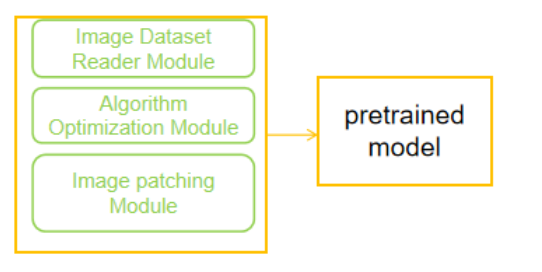
\includegraphics[width=0.4\textwidth]{train.png}
    \caption{Model Pretrain Process}
    \label{Fig4}
    \end{figure}

\subsection{Module}
MainFunction

\subsection{Uses}

\begin{itemize}
    \item Hardware-Hiding Module
    \item Input Upload and Validate Module
    \item Image Management Module
    \item Image Preprocessing Module
    \item Image Segmentation Module
    \item Output Format Module
    \item Report Generation Module
    \item User Interface Module
\end{itemize}

\subsection{Syntax}

\subsubsection{Exported Constants}
\begin{itemize}
    \item Max\_Upload\_Size: The maximum size allowed for image uploads.
    \item Supported\_Image\_Formats: A list of image formats that the system can process.
\end{itemize}

\subsubsection{Exported Access Programs}
1. System Initialization
\begin{itemize}
    \item Description: prepares the RVSS for operation, initializing subsystems, loading necessary resources, and setting up the environment for user interactions.
    \item Inputs: None
    \item Outputs: System status.
    \item Exceptions: ``InitializationException": raised if the system fails to initialize properly, possibly due to configuration errors or unavailable resources.
\end{itemize}

2. Start a new Session
\begin{itemize}
    \item Description: open a new user session, presenting the user interface and enabling access to the system's functionalities.
    \item Inputs: None
    \item Outputs: session identifier or status indicating a successful start.
    \item Exceptions: ``SessionStartException" raised if there's an issue initiating a new session.
\end{itemize}



3. Image Upload Process
\begin{itemize}
    \item Description: coordinates the upload of images by users, ensuring proper validation and storage for subsequent processing steps.
    \item Inputs: image files selected by the user.
    \item Outputs: confirmation of successful uploads, including identifiers (ImageID) for the uploaded images.
    \item Exceptions: ``ImageUploadException" Raised if an error occurs during the image upload process.
\end{itemize}

4. Execute Segmentation
\begin{itemize}
    \item Description: triggers the image segmentation process for the uploaded images, utilizing the Image Preprocessing and Image Segmentation Modules.
    \item Input: identifiers for images (ImageID) ready for segmentation.
    \item Output: status feedback during segmentation. Notification upon completion or if issues arise.
    \item Exceptions: ``SegmentationException": raised if the segmentation process encounters errors.
\end{itemize} 

5. Display Segmentation Results
\begin{itemize}
    \item Description: display the image segmentation result for the uploaded images.
    \item Input: identifiers for images (ImageID) already segmented.
    \item Output: Segmentation results, including any relevant data and metrics.
    \item Exceptions: ``ResultsDisplayException": raised if the display result process encounters errors.
\end{itemize} 

6. Generate Reports
\begin{itemize}
    \item Description: initiates the generation of comprehensive reports based on segmentation results, incorporating analytical insights.
    \item Inputs: identifiers for segmentation results to be included in reports.
    \item Outputs: the generated reports files.
    \item Exceptions: ``ReportGenerationException": raised if there are issues generating the reports.
\end{itemize}


\subsection{Semantics}

\subsubsection{State Variables}
\begin{itemize}
    \item Current\_Session: tracks information about the active user session. 
    \item Uploaded\_Images: maintains a list of images uploaded during the current session.
\end{itemize}

\subsubsection{Environment Variables}
\begin{itemize}
    \item System\_Config\_Path: specifies the path to system configuration files.
\end{itemize}


\subsubsection{Assumptions}
\begin{itemize}
    \item The system is operated in an environment with adequate computational resources.
    \item External services and modules (e.g., for image processing or report generation) are available and functional.
\end{itemize}



\subsubsection{Access Routine Semantics}

\noindent main():
1. Transition: Control the order of execution of different modules as follow:
\begin{itemize}
\item Upload Image
    \begin{itemize}
        \item  Module Used:  Input Upload and Validate  Module (M2, Section \ref{m1}), Image Management Module (M3, Section \ref{m2}), User Interface Module (M8, Section \ref{m7})
        \item Process: User selects image files for upload (M8, Section \ref{m7}). The  Input Upload and Validate  Module (M2, Section \ref{m1}) validates the file format and size. Images are uploaded and stored (M3, Section \ref{m2}), ready for preprocessing.
    \end{itemize}

    \begin{figure}[H]
    \centering
    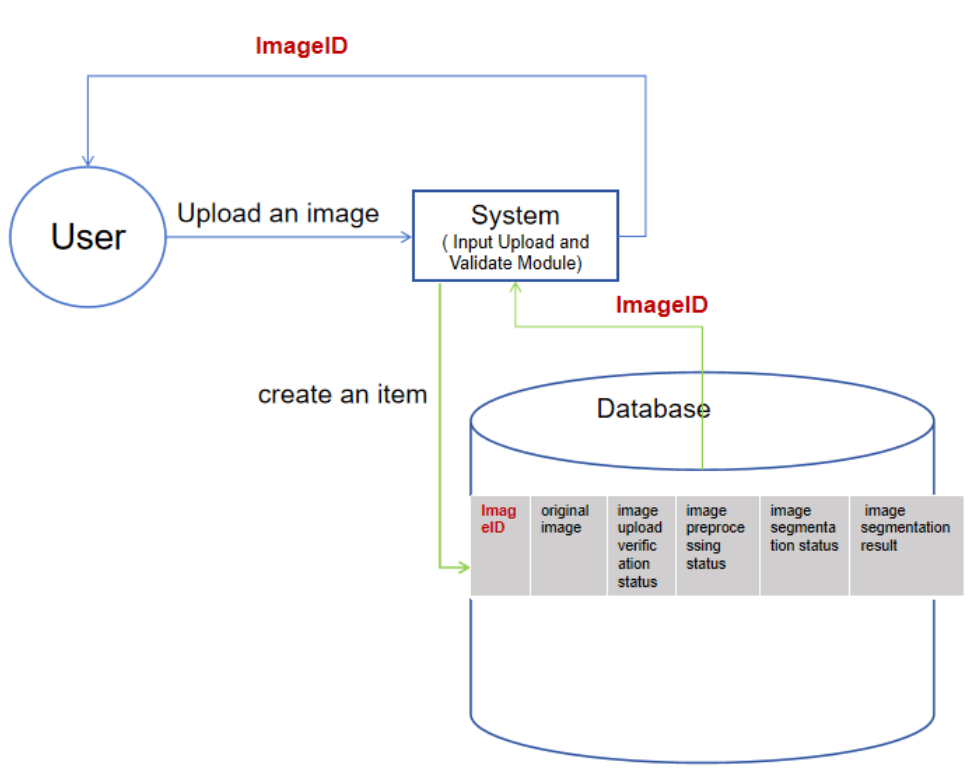
\includegraphics[width=0.5\textwidth]{upload.png}
    \caption{Upload Image}
    \label{Fig5}
    \end{figure}
\item Preprocess Image
    \begin{itemize}
        \item  Module Used: Image Management Module (M3, Section \ref{m2}), Image Preprocessing Module (M4, Section \ref{m3})
        \item Process: The Main Function Module sends uploaded images to the Image Preprocessing Module (M4, Section \ref{m3}). The images undergo preprocessing steps to enhance quality. Preprocessed images are stored with the ImageID  (M3, Section \ref{m2}), ready for segmentation.
    \end{itemize}
    
    \begin{figure}[H]
    \centering
    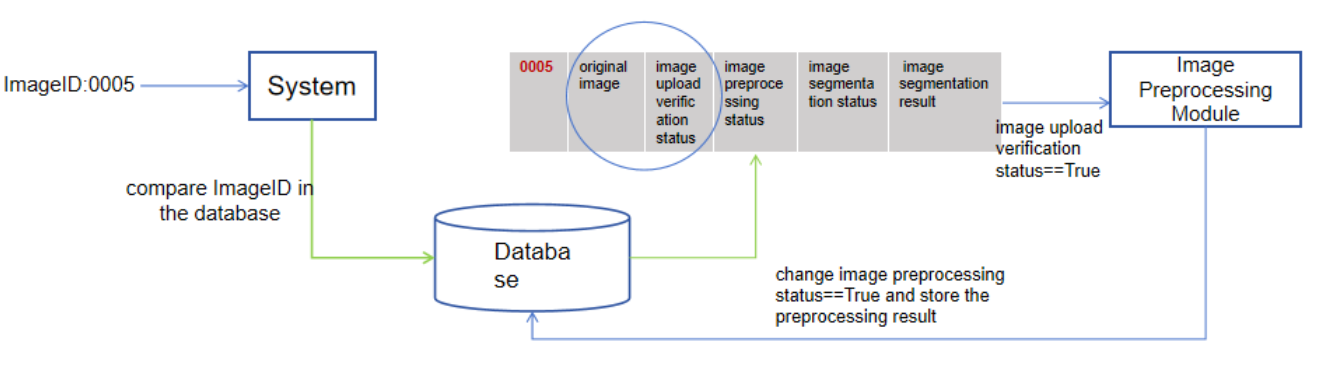
\includegraphics[width=0.6\textwidth]{preprocess.png}
    \caption{Preprocess Image}
    \label{Fig6}
    \end{figure}

\item Segment Image
    \begin{itemize}
        \item  Module Used: Image Management Module (M3, Section \ref{m2}), Image Segmentation Module (M5, Section \ref{m4})
        \item Process: Preprocessed images are then forwarded to the Image Segmentation Module (M5, Section \ref{m4}), where segmentation model has pre-trained. Segmentation model can identify and delineate retinal vessels.Preprocessed images are stored with the ImageID  (M3, Section \ref{m2}).
    \end{itemize}
    \begin{figure}[H]
    \centering
    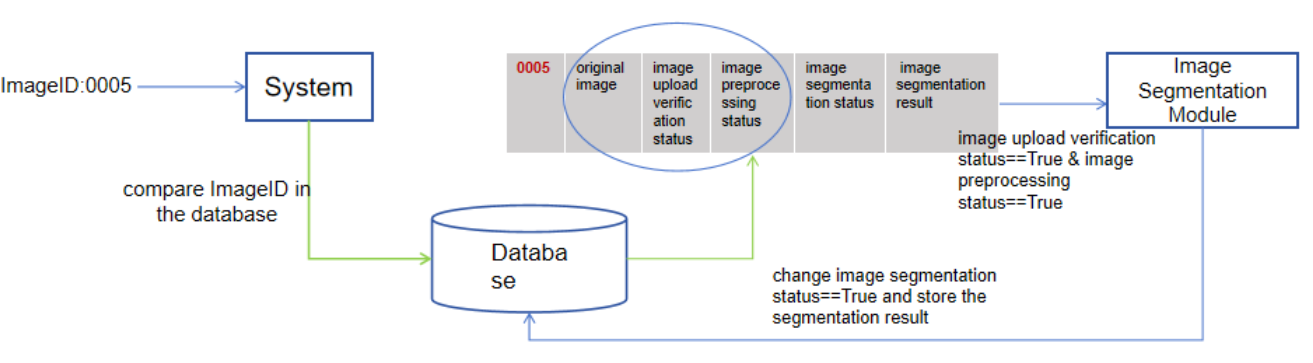
\includegraphics[width=0.6\textwidth]{seg.png}
    \caption{Segment Image}
    \label{Fig7}
    \end{figure}

\item Display Segmentation Result
    \begin{itemize}
        \item  Module Used: Image Management Module (M3, Section \ref{m2}), Output Format Module (M6, Section \ref{m5}),  User Interface Module (M8, Section \ref{m7})
        \item Process: use the ImageID to retrieve the segmented images and the main function module instructs the user interface module to display the segmentation results.
    \end{itemize}
    \begin{figure}[H]
    \centering
    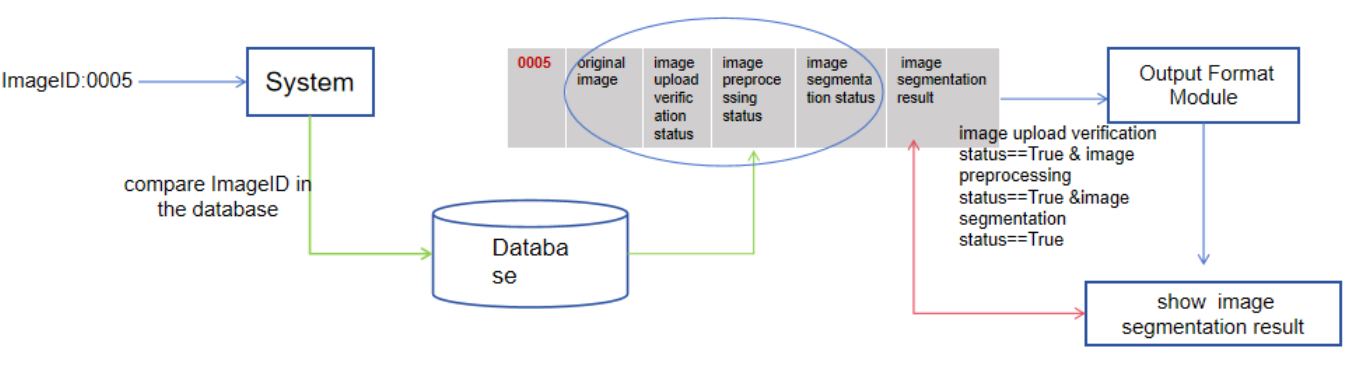
\includegraphics[width=0.6\textwidth]{display.png}
    \caption{Display Segmentation Result}
    \label{Fig8}
    \end{figure}

\item Generate Report
    \begin{itemize}
        \item  Module Used: Image Management Module (M3, Section \ref{m2}), User Interface Module (M8, Section \ref{m7}), Report Generation Module (M7, Section \ref{m6})
        \item Process: use the ImageID to retrieve the segmented images and the main function module instructs the user interface module to display the segmentation results.
        \item Segmentation results are collected according to the ImageID (M3, Section \ref{m2}). The Report Generation Module compiles these into a structured report (M7, Section \ref{m6}).
    \end{itemize}

\item Exception: Potential exceptions raises are from different sub-modules only.   
\end{itemize}


\subsubsection{Local Functions}

None

\newpage
\section{MIS of Plotting Result Module} \label{Plotting_Result_Module} 

\subsection{Module}
plot

\subsection{Uses}

\begin{itemize}
    \item Hardware Hiding Module
\end{itemize}

\subsection{Syntax}

\subsubsection{Exported Constants}
None

\subsubsection{Exported Access Programs}
1. Plot Segmentation Overlay
\begin{itemize}
    \item Description: generates a plot displaying the segmentation overlay on the original image, highlighting the segmented vessels.
    \item Inputs: the original fundus image ``OriginalImage" and the output from the segmentation process ``SegmentationResult", including the segmented vessel image.
    \item Outputs: an image ``OverlayPlot" with the segmentation results overlaid on the original image, suitable for visualization and assessment.
    \item Exceptions: ``PlottingException" raised if there is an issue generating the overlay plot.
\end{itemize}

2. Plot Segmentation Metrics
\begin{itemize}
    \item Description: visualizes various segmentation metrics in a graphical format, such as accuracy, sensitivity, specificity, or other relevant performance measures.
    \item Inputs: a collection of metrics data generated from the segmentation process.
    \item Outputs: a graphical representation (e.g., bar chart, line graph) of the segmentation metrics, facilitating easy interpretation of performance.
    \item Exceptions:``MetricsPlottingException": Raised if there is an error in plotting the metrics data.
\end{itemize}


\subsection{Semantics}

\subsubsection{State Variables}
\begin{itemize}
    \item Current\_Plot: Stores the most recently generated plot, which can be an overlay plot or a metrics plot.
\end{itemize}

\subsubsection{Environment Variables}
\begin{itemize}
    \item Plot\_Storage\_Path: specifies the directory where generated plots should be saved.
\end{itemize}

\subsubsection{Assumptions}
\begin{itemize}
    \item The segmentation results and metrics data provided to the module are accurate and in a format that can be processed for visualization.
\end{itemize}

\subsubsection{Access Routine Semantics}
1. Plot Segmentation Overlay
\begin{itemize}
    \item Transitions: The module combines the ``OriginalImage" and ``SegmentationResult" to create an overlay image where segmented vessels are clearly visible against the original background.
    \item Exceptions: ``PlottingException" raised if the overlay cannot be generated due to issues with input data formats, or incompatibilities.
\end{itemize}

2. Plot Segmentation Metrics
\begin{itemize}
    \item Transitions: The module takes metrics data and converts it into a visual format, choosing appropriate chart types (e.g., bar charts, line graphs) based on the data characteristics.
    \item Exceptions: ``MetricsPlottingException" raised if there are issues converting metrics data into graphical form, such as missing data points or unsupported data types.
\end{itemize}



\subsubsection{Local Functions}

None


\newpage
\bibliographystyle {plainnat}
\bibliography {ref}

\end{document}